\title{INTD262: Number Systems in pre-Columbian Context}
\author{Dr. Jordan Hanson - Whittier College Dept. of Physics and Astronomy}
\date{\today}
\documentclass[10pt]{article}
\usepackage[a4paper, total={18cm, 27cm}]{geometry}
\usepackage{outlines}
\usepackage{hyperref}
\usepackage{graphicx}
\begin{document}
\maketitle

\section{How to Submit this Assignment}

Once you answer the questions, take a picture of your work and convert it to a PDF.  Submit the PDF to the assignment link on Moodle.

\section{Review of Bases}

\begin{enumerate}
\item In the first video, we reviewed the base-10 number system.  As a warm up, express each of these numbers in \textit{expanded form}.  That is, show how each number is a sum of digits times powers of 10 (the first one is done as an example).
\begin{itemize}
\item $1024 = 1 \times 10^3 + 0 \times 10^2 + 2 \times 10^1 + 4 \times 10^0$
\item $2048 = $
\item $42 = $
\item $65,536 = $
\end{itemize}
\item Draw each of the numbers above as \textit{Quipu knot diagrams,} as shown in the first video. \\ \vspace{4cm}
\item Draw the following table of numbers as a \textit{Quipu knot diagram,} as discussed in the first and second videos.
\begin{table}[hb]
\centering
\begin{tabular}{| c | c | c |}
\hline
2 & 3 & 5 \\ \hline
7 & 11 & 13 \\ \hline
17 & 19 & 23 \\ \hline
\end{tabular}
\end{table}
\end{enumerate}

\section{Accounting Problems}

\begin{enumerate}
\item Suppose you are an Incan citizen who speaks Quechua, bringing a herd of \textit{guanaco} to the state office for re-distribution\footnote{Fascinatingly, the Inca had \textit{no concept of money.} A good idea for a final project would be to report on the Inca economic innovation of maintaining an empire without money.}.  You are adding thirteen guanaco to the office stables, and there are already twenty-five there.  How many are there in total?  \textit{Write the calculation in the Quipu notation.} \\ \vspace{3cm}
\item Suppose you are an Incan agricultural planner who is tasked with designing a farm terrace on a cliffside.  The architect informs you that there will be six plots of flat land created, each five by ten meters.  The six plots are at two altitudes, three high, three low.  The higher altitude is optimal for growing potatoes, while the lower altitude is better for squash.  A potato requires a square of earth one-half a meter on a side, while a squash requires a square of earth one-quarter a meter on a side.  \textit{Use Quipu knot notation} as a spreadsheet to determine how many squashes and how many potatoes can be planted.  \textit{There are many ways to create spreadsheets.  Just make sure to tell me how you would interpret your knots.}
\end{enumerate}

\begin{figure}
\centering
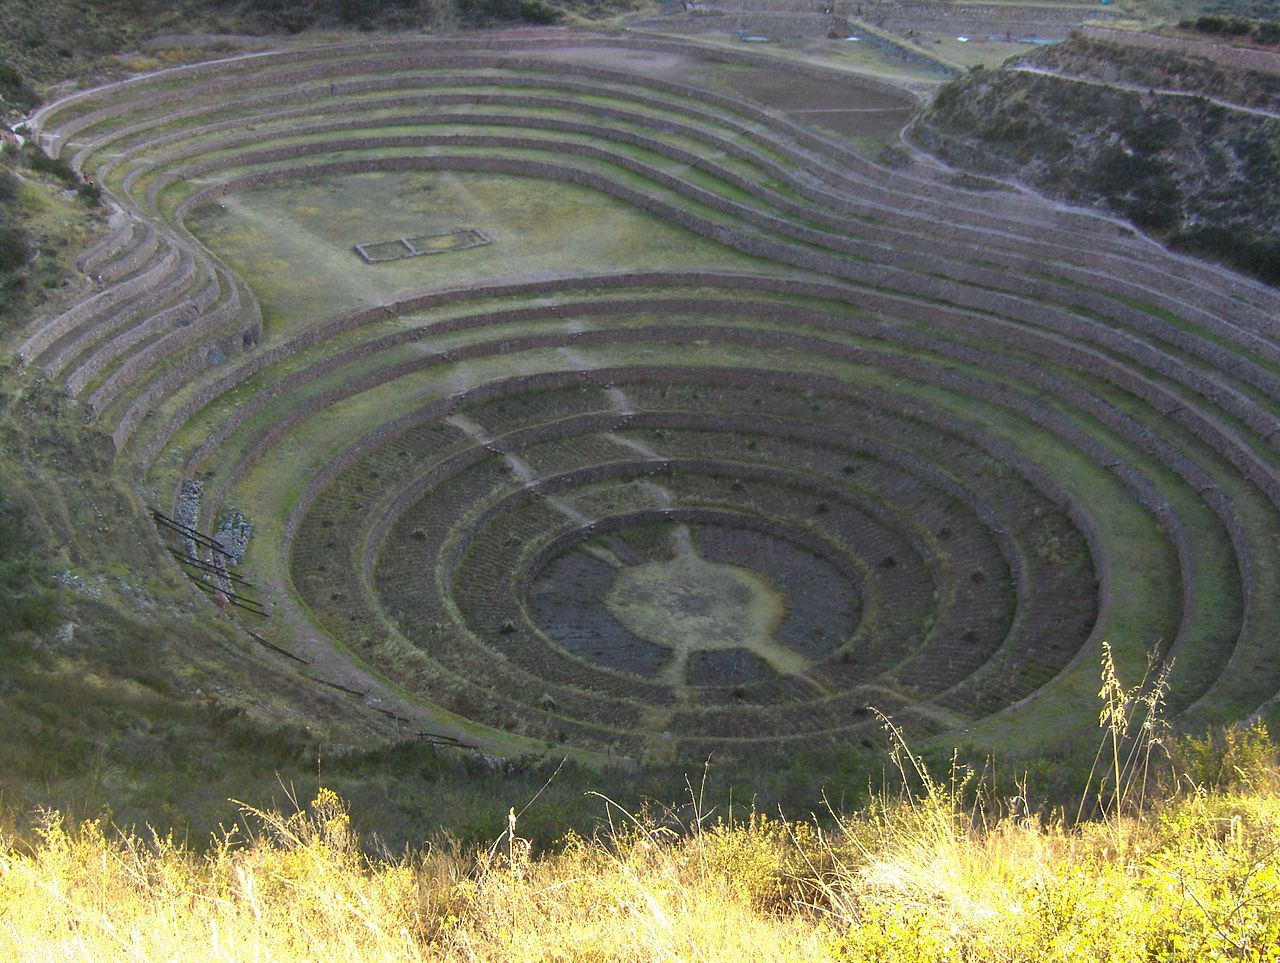
\includegraphics[width=7cm]{figures/terrace.jpeg}
\caption{An example of Incan terraces.}
\end{figure}

\end{document}
